\section{Individual Contribution}

\subsection{Member \#1}
\textbf{Student Index Number: } 21001792\\
\textbf{Student Name: } SAVINDA H.W.N.\\
\textbf{Components implemented:} 
\begin{itemize}
    \item Equipment management
    \item Orders management
    \item Rental Services search component
    \item Payment Gateway
\end{itemize}
\textbf{Description of the component(s):}
\begin{itemize}
    \item Equipment management – Rental Shops can add, update, view, remove, increase count, temporarily disable equipment from the inventory.
    \item Orders management – Customers can place orders, cancel orders and the rental shops can accept or reject the orders. The equipment will be mark as rented and returned later on.
    \item Rental Services search component – by inputting the location, item name and the date, customers can view the most relevant and available items to the search.
    \item Payment Gateway – Customer paying for orders
\end{itemize}






\subsection{Member \#2}
\textbf{Student Index Number: } 21000735 \\
\textbf{Student Name: } GUNAWARDENA R.S.U. \\
\textbf{Components implemented:} 
\begin{itemize}
    \item Dashboard of the admin
    \item Complaint management by admin
    \item Managing Tips and Knowhows 
\end{itemize}
\textbf{Description of the component(s):}
\begin{itemize}
    \item Dashboard of the admin – Statistical charts of users and bookings, Report generation of the income, view modification
    \item Complaint management by admin – Resolving complaints 
    \item Managing Tips and Knowhows – Add, delete, update Tips and Knowhows
\end{itemize}



\subsection{Member \#3}
\textbf{Student Index Number: } \\
\textbf{Student Name: } RAJAPAKSHA S.P.A.G.T.\\
\textbf{Components implemented:} 
\begin{itemize}
    \item Dashboards of Guide
    \item Guide profile and package management by Guide
    \item Guide Availability
    \item Guide Booking and Filter Guide by Customer
\end{itemize}
\textbf{Description of the component(s):}
\begin{itemize}
    \item Guide dashboard - The guide can view a brief summary of his bookings, including income, No of Tours, recent booking, upcoming booking, and the comparison between completed bookings and all bookings.
    \item Guide Profile and packages management - The guide can edit the profile of the Guide profile that the customer views and add, edit, and delete packages
    \item Guide Availability - Update Availability of the guide
    \item Guide Booking - The guide can view the booked days, and the customer can Filter and choose the relevant guide for the customer, select the package, and book the guide.
\end{itemize}







\subsection{Member \#4}
\textbf{Student Index Number: } \\
\textbf{Student Name: } SARANI H.A.S. \\
\textbf{Components implemented:} 
\begin{itemize}
    \item Customer complaint management
    \item Rental complaint management
    \item Login page and Signup page
    \item Customer frontend
\end{itemize}
\textbf{Description of the component(s):}
\begin{itemize}
    \item Customer Complaint Management : Customers can complain about rental services, Customers can view the all complaints they have made, Customers can view rejected complaints by admin
    \item Rental service Complaint Management : Rental services can view received complaints by customers and, resolve and reject complaints by admin, Rental services can complain to customers, Admin can resolve or reject complaints received by both customers and rental services
    \item Login and signup page, Customer frontend : frontend designs of all pages of the mentioned pages
\end{itemize}

\begin{figure}[h!]
    \centering
    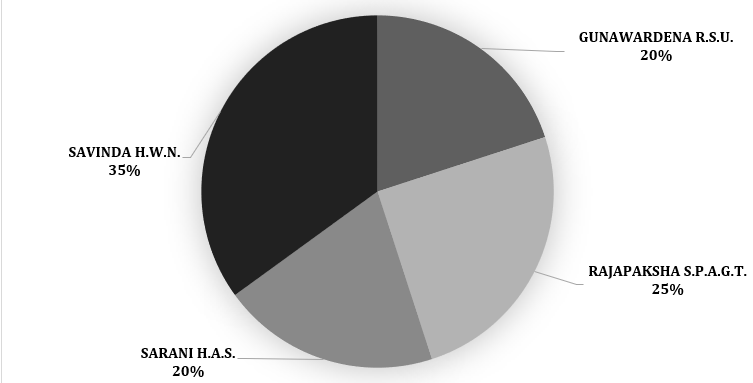
\includegraphics[width=1\textwidth]{Images/pie.png}
    \caption{ER diagram}
    \label{fig:enter-label}
\end{figure}
\clearpage




